\section{Introduction}
\label{sec:intro}



Conversational Agents (i.e., chatbots) are becoming increasingly popular in the mental health domain \cite{sabour2022chatbots}. Applications designed for mental health therapy or coaching in daily life, such as Woebot\footnote{\url{https://woebothealth.com}} and Wysa\footnote{\url{https://www.wysa.com}}, are gaining widespread attention for their ability to reduce users' negative emotions~\cite{Grove2021Codevelop} and promote a healthy lifestyle~\cite{Fadhil2019AssistiveCA}. Another notable application is chatbot-based symptom checkers~\cite{Yue2023Beyond}, which emulate human-like conversations while assessing users' symptoms, resembling interactive questionnaires.
% for their ability to help users manage their emotions and provide useful suggestions based on various techniques such as cognitive behavior therapy (CBT) and meditation. (psychological therapy)
 % \KZ{There's too little detail about the two bots. Can you say a bit more?} 

However, there is still limited exploration in developing and evaluating chatbots that can (i) conduct diagnosis conversations like a psychiatrist
or (ii) simulate patients in the psychiatric outpatient scenarios, though they have significant real-world applications. 
Doctor chatbots can be effective tools for mental disorder screening~\cite{pacheco2021Smart} in lieu of official medical diagnosis. Patient chatbots can serve as Standard Patients (SP) in medical education, making the process more efficient and cost-effective~\cite{Torous2021growing}.

Developing and evaluating such chatbots is particularly challenging due to the unique nature of mental health issues, including (i) the difficulty in obtaining data because of privacy concerns; (ii) the inherent ambiguity and subjectivity of mental disease symptoms. 
% COMMENT: privacy *between*?
Moreover, relying solely on scales (e.g., PHQ-9) for mental disorder screening cannot provide trustworthy diagnosis, because in real outpatient scenario, patients often feel ashamed or afraid of disclosing their true conditions and difficult to describe their mental state objectively~\cite{Salaheddine2016Identify}. 
% Thus, even experienced psychiatrists struggle to obtain the meaningful response from patients. 
% \MY{This sentence is a bit awkward, i know what you mean but what psychiatrists do is still asking questions. Consider saying that why questionnaires and scales cannot  because in real outpatient scnenario that xxx}

Consequently, the design goals and conversational styles of these chatbots are different from the chatbots for mental health therapy and symptom checking.
% COMMENT: 这里对chatbots for therapy和task-oriented chatbots的特征再多说一点是否更好,否则怎么知道他们不同在哪儿呢?
We argue that chatbots for psychiatric diagnosis can not achieve satisfying performance by simply collecting symptoms like questionnaires. Instead, they should be equipped with various professional skills, such as emotional support, to complete the diagnosis task effectively.
What's more, patient chatbots should aim to resemble real patients more closely, rather than precisely and robotically reporting their symptoms without any emotional fluctuations.

\begin{figure*}[th]
	\centering
	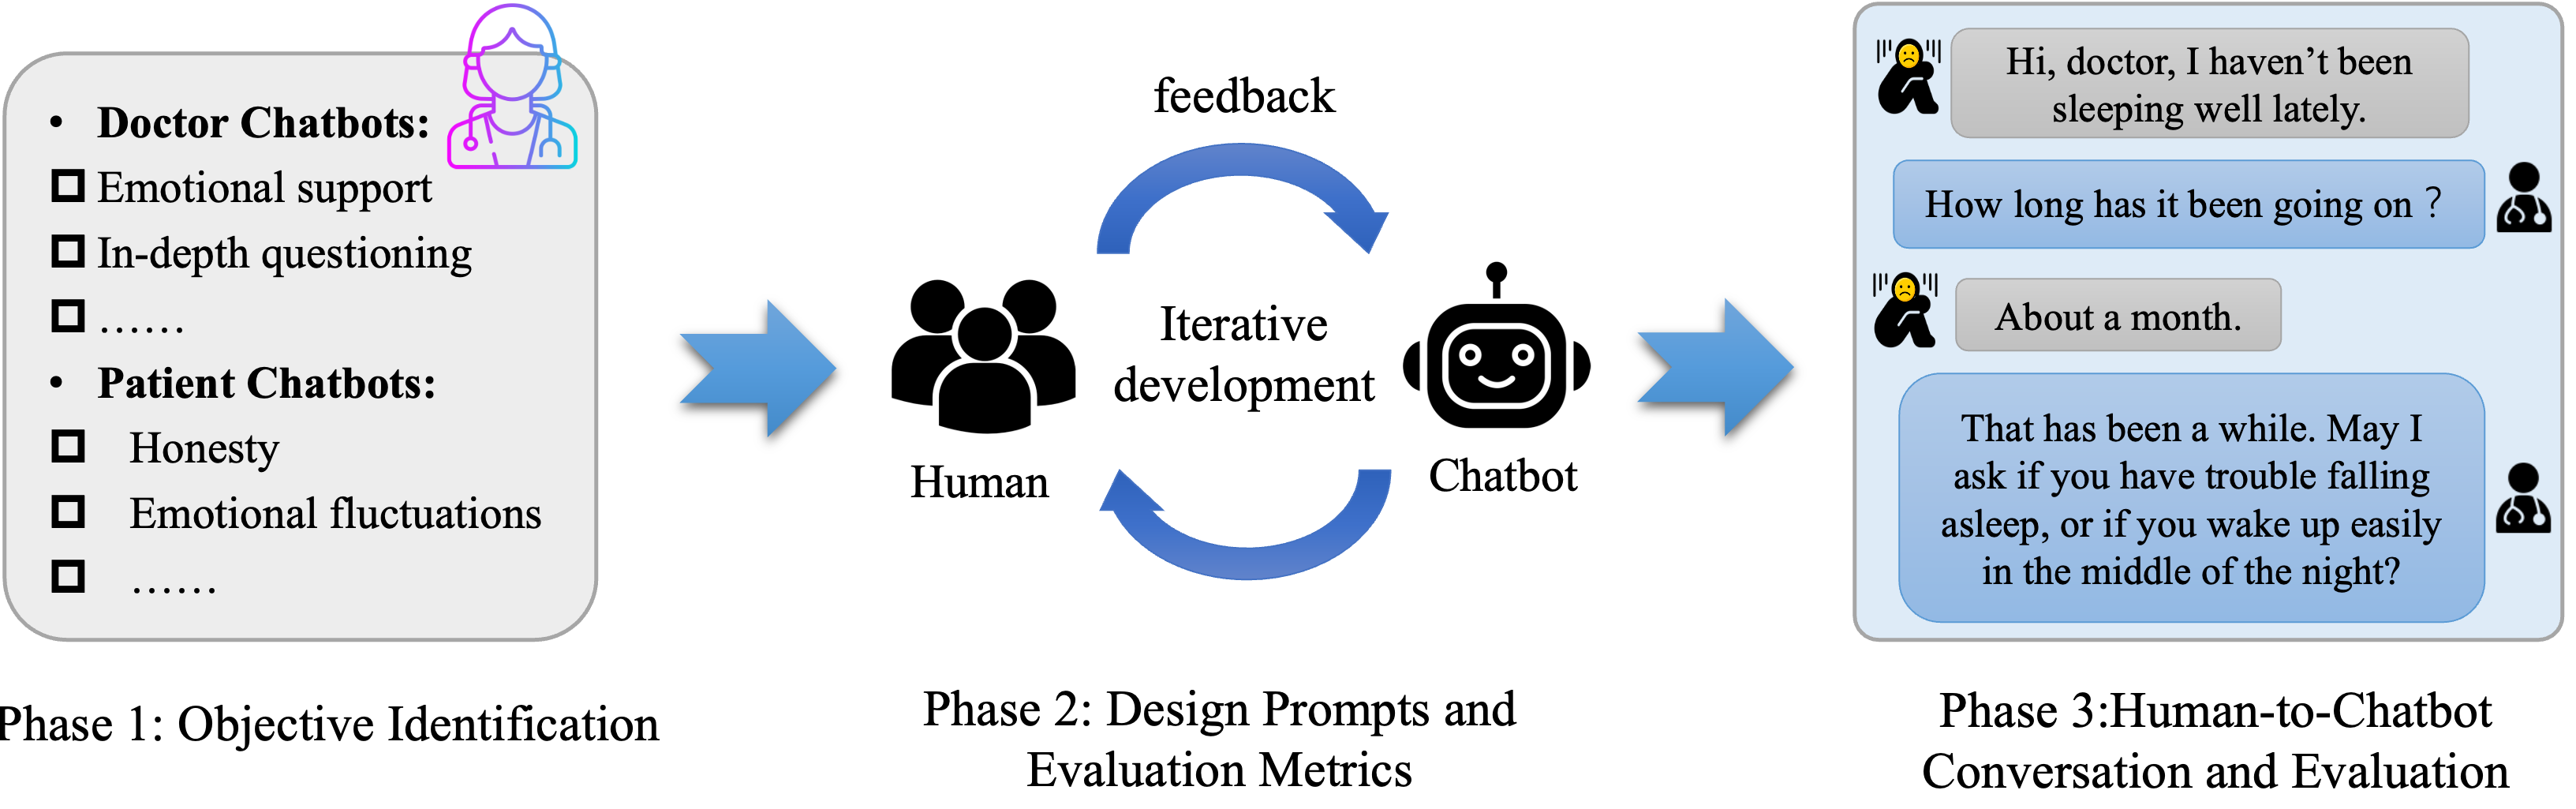
\includegraphics[width=0.8\linewidth]{Figures/overview.png}
	\caption{The overview of the psychiatrist-guided three-phase study.}
	\label{fig:pipeline}
\end{figure*}

% However, many existing frameworks~\cite{Medeiros2018UsingCF,Jaiswal2019Virtual} still rely on rule-based approaches (e.g., utilize the questions in self-rating scales), which often result in rigid conversations and cannot show sufficient empathy to patients. Alternatively, other deep learning methods \cite{yao-etal-2022-d4} require a significant amount of domain-specific data for training, which is often costly and difficult to obtain, especially in the mental health domain. 
% Furthermore, due to the diverse ways to express mental states verbally, neither rule-based nor data-based methods can comprehensively cover all possible cases, so the patient chatbots developed using these methods tend to be inflexible and lack diversity~\cite{Yao2020Toward}.

% \KZ{But how is simulating doctors and patient in diagnosis conversation more difficult than the therapeutic bots in Woebot and Wysa, and the like? In other words, why can't we use the techniques in Woebot and Wysa to simulate doctors and patients? I think the difference between diagnostic bots and therapeuric bots is that it's easier to verify quality of the doctor bot or patient bot: a good doctor bot must be able to acquire enough info efficiently from the patient so as to make a correct diagnosis; a good patient bot must resemble the real patient in doctors eyes. A good therapist however can't be easily qualified because all they are doing is to make the patient feel better, which is very subjective from the patient point of view.}  

Achieving these goals is quite difficult for conventional rule-based~\cite{Medeiros2018UsingCF,Jaiswal2019Virtual} or data-based~\cite{yao-etal-2022-d4, Fansi2022DDXPlus, Lin2021Graph} methods. Fortunately, recent advancements in large language models (LLMs), especially with the emergence of ChatGPT\footnote{\url{https://chat.openai.com/}}, provide a new way to develop chatbots that can convincingly portray specific roles.  Equipped with comprehensive training data and knowledge, LLMs can generate diverse tones and symptom descriptions with appropriate prompts rather than fine-tuning on extensive domain data.
% \KZ{Can ChatGPT be used to simulate therapeutic bots as well?}  
% COMMENT: 前面所述,该chatbot的困难有两点:数据难采集和症状的模糊、主观。这里只讲清楚了ChatGPT能够解决数据采集的问题,那么它怎么来应对症状模糊主观的问题呢?此外还包括刚才上一段提到的,diagnosis chatbot需要提供情感支撑,patient simulator要仿真病人的情绪波动,要如何实现,这里是不是都应该简单描述一下?

Therefore, in this work, we aim to (i) respectively investigate the potential of ChatGPT in simulating psychiatrists and mental disordered patients in a clinical diagnosis scenario\footnote{For the sake of clarity, we will refer to these two types of chatbots as the \textbf{``doctor chatbot''} and \textbf{``patient chatbot''} respectively in the subsequent sections.}, 
% \MY{maybe more clearly: in simulating \textit{psychiatrists} and \textit{mental disordered patients} in a clinical diagnosis scenario. For the sake of ...}
as well as (ii) build a comprehensive evaluation framework for these chatbots, answering the question about what constitutes an exceptional psychiatrist chatbot and a truly patient-like chatbot.

To develop and evaluate a system that truly satisfies users' expectations, we followed a human-centered design methodology. The study consists of three phases (See Figure~\ref{fig:pipeline}).
We first collaborated with psychiatrists to identify a set of objectives for doctor and patient chatbots (\textbf{Phase 1}). 
Based on these objectives, we conducted an experimental study (\textbf{Phase 2}) to design appropriate prompts for ChatGPT-based chatbots and establish an evaluation framework that incorporates both human evaluation and automatic metrics aligned with the objectives from Phase 1. Importantly, the design of prompts and metrics was iterated based on human feedback, with each version evaluated and improved with input from psychiatrists.
% COMMENT: 这里这个user feedback是专指psychiatrists吗?还是包含patients?感觉要明确一下

Further, to better evaluate the performance of these chatbots with varying prompt designs, we recruit real psychiatrists and patients to engage in diagnostic conversations with the simulated patient and doctor chatbots, respectively, and collect their ratings after conversation (\textbf{Phase 3}). We also conduct a comparison between the behavior of real and simulated psychiatrists based on the dialogue history, which yields some interesting findings. 
The main contributions of this work are:
\begin{itemize}
    \item We formalize the task of developing doctor and patient chatbot for diagnostic purposes in a psychiatric outpatient setting.
    \item We conduct a user-centered design and evaluation of these chatbots. Through an iterative development process, we actively sought feedback from both patients and psychiatrists, allowing us to establish a more (solid and applicable!!!) chatbot system and evaluation framework. 
    % \MY{thought we also have real patients' feedback during the process?} 
    % \MY{better emphasize that we create this pool of doctors and patients, and we can further situate our work part of RLHF with the ``H'' humans, where both ends' feedbacks are included}
    \item Through (detailed!!!) prompt engineering and experiments, we demonstrate the feasibility of utilizing ChatGPT-powered chatbots in professional domains that demand specialized skills or unique language style. We also use interactive human evaluation to explore how different prompt designs influence user experience. (show results+data) %(diag acc + efficiency + human-like + user experience +强调比baseline更接近人)
    % for psychiatric diagnosis and patient simulation, as well as explore its possible limitations. We also find that different prompt designs can have an impact on the behavior and language style of chatbots, ultimatly influencing the users' experience. 
    % \item We suggest a data augmentation strategy that employs carefully evaluated doctor and patient chatbots to produce unlimited psychiatric outpatient dialogue data, effectively tackling the obstacle of obtaining data due to ethical concerns in mental health domain. We also provide the dataset containing dialogues between chatbots and real patients or psychiatrists from our evaluation experiments, which has been anonymized for privacy. 
    % \KZ{Ethical and privacy concerns?}
\end{itemize}




% Intuitively, relying on traditional evaluation metrics for dialogue systems (e.g., n-gram overlap, semantic textual similarity) to assess the performance of doctor and patient chatbots in mental health scenarios is inadequate, as there is no standardized answer for clinical conversations. 
% Moreover, what constitutes an exceptional psychiatrist chatbot or a realistic patient chatbot still remains unexplored. 

